%%%%%%%%%%%%%%%%%%%%%%%%%%%%%%%%%%%%%%%%%%%%%%%%%%%%%%%%%%%%%%%%%%%%%%%%%%%
% Definitions                                                             %
%%%%%%%%%%%%%%%%%%%%%%%%%%%%%%%%%%%%%%%%%%%%%%%%%%%%%%%%%%%%%%%%%%%%%%%%%%%
\gdef\version{0.1}
\gdef\doctype{Businessplan}

\documentclass[11pt]{article}
%Gummi|065|=)
\usepackage{graphicx}
\usepackage{color}
\usepackage[dvipsnames]{xcolor}
\usepackage{tabu}
\usepackage{fancyhdr}
\usepackage{titlesec}
\usepackage{lastpage}
\usepackage[utf8]{inputenc}
\usepackage{eurosym}
\usepackage{tabulary}
% headers
\renewcommand{\headrulewidth}{0.4pt}
\renewcommand{\footrulewidth}{0.4pt}
\renewcommand{\arraystretch}{1.4}
\fancyhead{}
\fancyfoot{}
\pagestyle{fancy}
\lhead{{\doctype}}
\rhead{{\fontfamily{phv}\selectfont \textcolor{gray}{Urban Green}} 
\includegraphics[height=0.8cm]{logo}}
\lfoot{Version \version}
\rfoot{\thepage\ von \pageref{LastPage}}
\setlength{\headheight}{30pt}

%%%%%%%%%%%%%%%%%%%%%%%%%%%%%%%%%%%%%%%%%%%%%%%%%%%%%%%%%%%%%%%%%%%%%%%%%%%
% Document Start                                                          %
%%%%%%%%%%%%%%%%%%%%%%%%%%%%%%%%%%%%%%%%%%%%%%%%%%%%%%%%%%%%%%%%%%%%%%%%%%%

\begin{document}

\begin{titlepage}
    \centering
    \vfill
    {
        \Huge\textbf{Businessplan}\\
        \vskip2cm
        
\includegraphics[width=4cm]{logo} \\
        \Large
        {\fontfamily{phv}\selectfont
			\textcolor{gray}{Urban Green}%
		}
        \vskip3cm
        Matthias Schwebler\\
        Ramin Bahadoorifar\\
        Samuel Schober\\
        Konrad Kelc\\
    }
    \vfill
    \begin{center}
    \begin{table}[ht]
    	\centering
    	\begin{tabular}{lllll}
    		\cline{1-4}
    		\multicolumn{1}{|c|}{\textbf{\rule{0pt}{3ex} }} & \multicolumn{1}{c|}{\textbf{Name}} & \multicolumn{1}{l|}{\textbf{Datum}} & \multicolumn{1}{l|}{\textbf{Unterschrift}} &  \\ \cline{1-4}

    		\multicolumn{1}{|l|}{\textbf{\rule{0pt}{3ex} Erstellt:}} & \multicolumn{1}{l|}{M. Schwebler, R. Bahadoorifar} & \multicolumn{1}{l|}{2.11.2016} & \multicolumn{1}{l|}{} &  \\ \cline{1-4}

    		\multicolumn{1}{|l|}{\textbf{\rule{0pt}{3ex} Gepr\"uft:}} & \multicolumn{1}{l|}{S. Schober, K. Kelc} & \multicolumn{1}{l|}{2.11.2016} & \multicolumn{1}{l|}{} &  \\ \cline{1-4}
    		&  &  &  &  \\
    		&  &  &  &  \\
    		&  &  &  &  \\
    	\end{tabular}
    \end{table}
    \end{center}
\end{titlepage}

\section{Executive Summary}
\subsection{Die Idee}
Unsere Produktidee ist, dass wir ein automatisiertes Aquaponiksystem entwickeln, welches die Beobachtung der Parameter, wie zum Beispiel Hitze, Wasserstand und PH-Wert, dem Benutzer abnimmt und somit den Gebrauch, eines Aquaponiksystems, erleichtert. Unser Bestreben ist, dass wir durch unser Homeponicsystem eine Alternative zu den herkömmlichen Methoden, der Beschaffung von Obst, Gemüse und Kräutern, bieten und somit das Kaufverhalten, bezüglich saisonalem, beziehungsweise massenproduziertem, Obst und Gem\"use, unserer Kunden so ändern, dass weniger importiertes Obst/Gemüse gekauft wird. Unser wichtigstes Alleinstellungsmerkmal ist, dass wir als einziges Unternehmen in \"Osterreich ein automatisiertes Aquaponiksystem anbieten können.
\subsection{Das Team}
Das Urban Green Team setzt sich aus 4 Mitgliedern zusammen:
\begin{itemize}
    \item Bahadoorifar Ramin
    \item Kelc Konrad
    \item Schober Samuel
    \item Schwebler Matthias
\end{itemize}
Die Schwerpunkte unseres Projektes verteilen sich auf die softwaretechnische und die hardwaretechnische Umsetzung. Durch unsere vierjährige Ausbildung, in der Abteilung IT, des TGM, haben alle Mitglieder unseres Teams genug Erfahrung in dem softwaretechnischen Bereich. Der hardwaretechnische wird mit Hilfe unseres Kooperationspartners Ponix Systems GmbH realisiert.
\subsection{Kooperation}
Wie erwähnt, wird eine Kooperation mit der Ponix Systems GmbH eingegangen, welche durch ihre Forschung und Entwicklung eines automatisierten Hydroponiksystems schon viel Know How mit in unser Projekt eingebracht haben.
\subsection{Das Unternehmen}
Der Kunde bekommt nach Anfrage alle nötigen Informationen bzgl. des Kaufs, wie die AGB, Kaufauftragdokumente, etc., zugesendet und der Bestellauftrag wird nach Rücksprache, mit unserem Kauf-Support, durchgeführt und in der Fertigung in Auftrag gegeben. Danach bekommt der Kunde das bestellte Produkt, inklusive eines Handbuches, angeliefert.
\subsection{Die Vermarktung}
Unsere Zielgruppe sind Leute welche sich gerne gesund und ökologisch ernähren und nach einer Möglichkeit suchen, falls kein Garten vorhanden oder  das Obst-, die Gemüsesorte außerhalb der Saison ist, ihr eigenes Obst, Gemüse und Kräuter anzubauen. Weiters gibt unser Produkt botanisch interessierten Personen sehr viele Möglichkeiten mit Pflanzen zu experimentieren, da die von Ponix Systems GmbH entwickelte LED-Beleuchtung, mit ihren verschiedenen Wellenlängen, die Eigenschaften der Pflanze von Grund auf ändern kann. Dadurch lässt sich zum Beispiel der Geschmack, die Dauer des Wachstums oder die Größe der Pflanze beeinflussen.

Durch Werbung auf verschiedenen sozialen Medien und anderen Internet-Plattformen erhoffen wir uns, durch die häufige Internetaktivität, der an Aquaponik interessierten Konsumenten, ein gewisses Interesse in der Aquaponiker-Gemeinschaft zu erlangen, sodass wir durch den erfolgreichen Verkauf unseres Produkts, eine Werbekampagne auf anderen Medien starten können.
\subsection{Der Erfolg}
Evaluierung noch ausstehend.
\clearpage
\section{Unternehmen \& Management}
\subsection{Informationen zum Unternehmen}
Unsere Firma Urban Green wird vorraussichtlich Ende April 2017 gegründet.

Als Rechtsform wird wahrscheinlich eine GmbH gewählt weil diese, von allen Projektmitgliedern, als beste Option angesehen wird. Weiters wird das Eigentumsverhältnis wohlmöglich unter dem Projektteam gleichenteils aufgeteilt. Vertragliche Vereinbarungen sind diesbezüglich jedoch noch nicht bekannt.
Als Kooperationspartner haben wir Ponix Systems GmbH.
Durch die Kooperation werden diese Vorteile bereitgestellt:
\begin{itemize}
    \item Hardware, Single Board Computer, Aquarium, etc.
    \item Software, Ansteuerung von Sensorik ist Teils vorhanden
    \item Wissen, welches durch ein ähnliches Projekt erhoben wurde, das ebenso bereitgestellt worden ist
\end{itemize}
\subsection{Status der Unternehmensgründung}
Es wurden bislang noch keine wesentlichen Schritte bezüglich der Unternehmensgründung unternommen.
\subsection{Firmensitz}
Der Firmensitz ist bislang unbekannt
\subsection{Unternehmensanalyse}
Die Kernaufgabe unseres Unternehmens ist es Leuten, welche keinen Garten besitzen, das Anbauen von Obst, Gemüse und Kräutern im eigenem Wohnraum zu ermöglichen. Weiters ermöglichen wir das Anbauen in unwirtlichen Jahreszeiten.
Als Risiko ist bei uns die Möglichkeit vorhanden, dass die US-amerikanische Firma \textit{Grove Ecosystem} in den europäischen Markt einsteigt und unser Produkt nicht mehr einzigartig ist, da die Firma sich das selbe Ziel gesetzt hat. Jedoch erscheint uns das als geringes Risiko, da die Preise für solche Systeme oft im vierstelligem-Bereich liegen.
\subsection{Ziele}
Derzeit steht noch nicht fest ob wir das Produkt an eine andere Firma weitergeben oder von uns weitergeführt wird, da wir uns noch in der Forschung bzw. Entwicklung befinden.
\subsection{Unterstützung und Hilfestellung}
Personell werden wir von Alvaro Lobato und Prof. Schabel betreut, Ideell werden wir von Herrn AV. Koppensteiner, Alvaro Lobato und Prof. Schabel unterstützt finanziell erhalten wir Unterstützung, durch Bereitstellung von Materialien und Software, von Ponix Systems GmbH.
\subsection{Gründungsteam}
Wie erwähnt setzt sich das Urban Green Team aus 4 Mitgliedern zusammen.
Die Schwerpunkte unseres Projekts verteilen sich auf die softwaretechnische und die hardwaretechnische Umsetzung. Durch unsere vierjährige Ausbildung, in der Abteilung IT, des TGM, haben alle Mitglieder unseres Teams genug Erfahrung in dem softwaretechnischen Bereich. Weiters erlangten wir durch das TGM einige Erfahrung im Bereich Projektmanagement.
Unserem Team fehlt es an Erfahrung im Gebiet der Hardwareentwicklung, jedoch bekommen wir durch unseren Partner hier Hilfestellung.
Unser Team hat durch die Betreuung in der Abteilung IT die Fähigkeit erlangt gut in Teams zusammen zu arbeiten und weil wir uns schon seit über einem Jahr kennen und uns gut verstehen können wir gut miteinander arbeiten.
Samuel Schober ist in unserem Projekt der Product Owner und trägt dadurch die Aufgabe der Interessensvertretung des Projektteams nach Außen. Die restlichen Mitglieder, Bahadoorifar Ramin, Kelc Konrad und Schwebler Matthias, sind hauptsächlich für die Entwicklung des Homeponicsystems und der WebApp zuständig.
\clearpage
\section{Produktidee}
\subsection{Kundenbed\"urfnisse und Probleml\"osung}
Urban Green bietet in \"Osterreich die bisher nicht erh\"altlichen Produkte aus dem Hydroponik Bereich f\"ur den durchschnittlichen Haushalt. Der Kunde kann ein Aquaponic System, welches sonst nur in Betrieben im
großen Ausmaß, durchgef\"uhrt wird, bei sich Zuhause hobbym\"aßig betreiben. Dies kann man von den bereits bestehenden Heiml\"osungen nicht behaupten: Sie sind entweder gesetzlich nicht erlaubt oder in \"Osterreich nicht erh\"altlich.\\
\\ Das System bietet eine vollst\"andige \"Uberwachung des Ökosystems, mithilfe von PH-, EC- und Temperatursensoren. Des Weiteren kann das System vom Benutzer gesteuert werden, indem er Aktoren (Hitzestrahler, Futterautomat und Beleuchtung) \"uber die, von uns entwickelte, Web-Applikation steuert:
\\ \"Uber die Webapp, kann der Benutzer alle Daten der bisher genannten Sensoren und dessen Interpretationen ablesen und gegebenenfalls \"uber Steuerung der Aktoren Maßnahmen ergreifen. \"Uber die Webapp soll der Benutzer auch, bevor er sein Aquaponic System Fischen best\"uckt, ein breites Spektrum an Informationen \"uber m\"ogliche Kombinationen erhalten um eine, f\"ur ihn, optimale Besetzung des Aquariums und des Beetes zu erzielen. Er soll auch eigene "Profile" erstellen k\"onnen und andere Bewerten k\"onnen. So w\"achst das Portal, lediglich durch die Verwendung der Benutzer.
\newpage
\subsection{Produkte und Dienstleistungen}
Das Endprodukt ist ein Aquaponic System (Aquarium + Beet f\"ur Anbau), welches \"uber eine Website \"uberwacht bzw. gesteuert werden kann. Dazu z\"ahlen Daten wie: Wassertemperatur, EC-Wert, PH-Wert, Wasserstand, Belichtungsdauer und Intensit\"at der Beleuchtung.
\begin{center}
	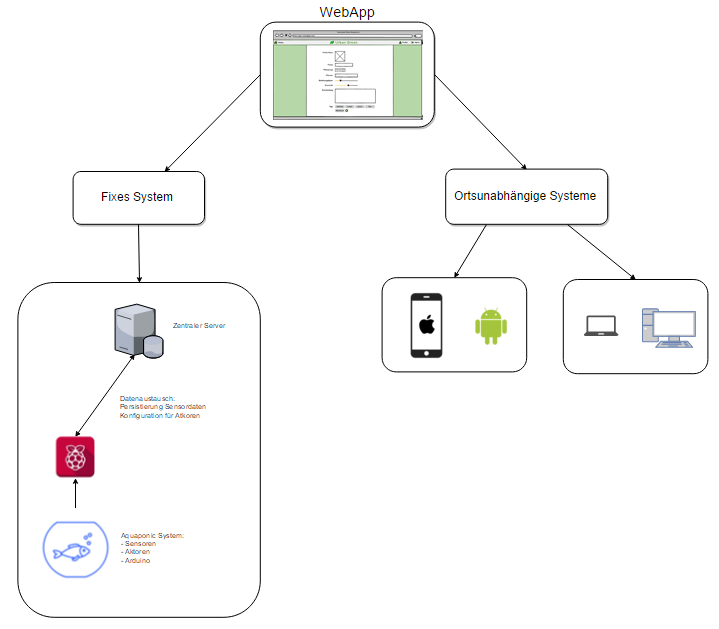
\includegraphics[width=12cm]{produkte}
\end{center}
\subsubsection{WebApp}
Besitzer eines Urban Green Aquaponic Systems, bekommen alle Daten der Sensoren in aufbereiteter Form, auf der WebApp zur Verf\"ugung gestellt. \"Uber die Website kann aber nicht nur abgelesen werden, sondern auch Konfigurationen f\"ur die Aktoren angepasst werden. \\
Neben den Echtzeitinformationen, k\"onnen auch Erfahrungswerte anderer Benutzer, bez\"uglich der Kombinationen von Fisch und Pflanzen gelesen und bewertet werden. So w\"achst das Portal stetig durch die Benutzung der Kunden. \\
Da das Produkt f\"ur die Marktl\"ucke in \"Osterreich und Deutschland konzipiert ist, wird die Website vorerst nur in Deutsch betrieben.
\subsubsection{Fixes System}
Das Aquarium und das Beet stellen das fixe System dar. Enthalten sind: Sensoren, Aktoren sowie ein Arduino und ein Raspberry Pi. Der Arduino \"ubernimmt die Schnittstelle zu den Sensoren. Er sendet in regelm\"aßigen Abst\"anden die Daten aller Sensoren an den Raspberry Pi und \"andert die Werte f\"ur die Aktoren (falls neue Konfiguration des Benutzers vorhanden). Der Raspberry Pi \"ubernimmt die sichere Kommunikation mit einem zentralen Server. Er sendet die Daten und fragt gleichzeitig neue Konfigurationen f\"ur die Aktoren ab. Sollte der Server nicht erreichbar sein, speichert er die Daten lokal zwischen, und \"ubertr\"agt sie bei Wiederherstellung der Verbindung.
\begin{center}
	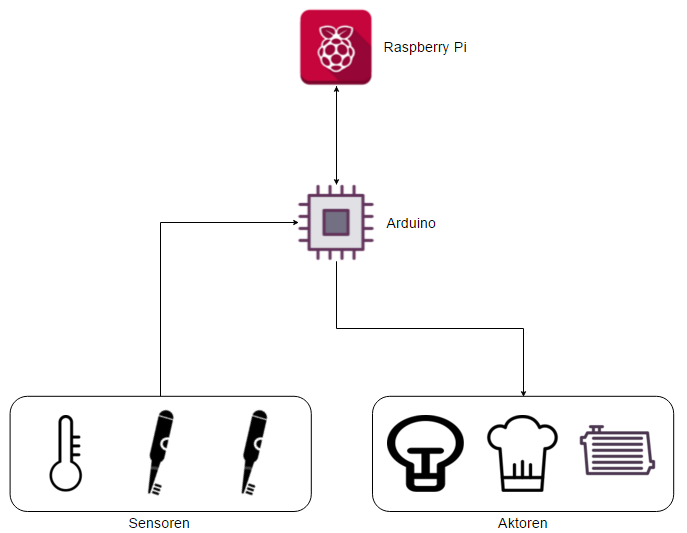
\includegraphics[width=8cm]{fixesSystem}
\end{center}
\vskip1cm
\begin{itemize}
	\item \textbf{Raspberry Pi}: Kommunikation mit Server, Zwischenspeicherung bei Netzausfall
	\item \textbf{Arduino}: Ansteuerung der Sensoren und Aktoren, \"Ubertragung der Daten an den Raspberry Pi
	\item \textbf{Sensoren}: Temperatur, PH-Wert, EC-Wert, Wasserstand
	\item \textbf{Aktoren}: Beleuchtung der Pflanzen, Futterautomat, Hitzestrahler
\end{itemize}
\subsubsection{Ortsunabh\"angige Systeme}
Da mobile Ger\"ate mittlerweile so verbreitet sind, dass sie bei nahezu jedem anzutreffen sind, ist die Schnittstelle des Systems zum Benutzer eine Website. Dies bietet den Vorteil, dass nur eine Applikation erstellt werden muss, die sowohl auf PCs, Laptops und Smartphones funktioniert. So kann der Benutzer auch, weit weg von zuhause auf sein Aquaponik System zugreifen.
\subsection{Einzigartigkeit in \"Osterreich}
Aquaponic Systeme sind haupts\"achlich im gr\"o{\ss}eren Ma{\ss}stab bei der Aufzucht von Nutzpflanzen im Einsatz. F\"ur den normalen Haushalt gibt es allerdings bis jetzt keine Marktf\"ahige L\"osung. Die gr\"o{\ss}ten zwei Crowdfunding Projekte sind:
\begin{itemize}
	\item \textbf{EcoQube C}\\
	Der EcoQube C vereint ein Handliches Aquaponics System mit elegantem Design, jedoch mangelt es an Konfigurierbarkeit. Es steht lediglich eine Fernbedienung zur verf\"ugung, mit der die Farbe der LEDs gesteuert werden kann. Des Weiteren liegt das Fassungsverm\"ogen des Aquariums weit unter 50 Liter, was zur Folge hat, dass in \"Osterreich maximal ein einziger Fisch darin gehalten werden kann. Daraus resultiert ein sehr kleines, ineffizientes Aquaponics System mit Mangel an Konfigurationsm\"oglichkeiten. \\
	\item \textbf{Grove Ecosystem}\\
	Das Grove Ecosystem ist das "Non Plus Ultra", wenn es um Aquaponic Systeme im Haushalt geht. Es bietet alle m\"oglchen Sensoren (Luftfeuchtigkeit und -temperatur sowie Wasserstand und -temperatur), welche \"uber eine App abgefragt werden k\"onnen. Diese bietet zus\"atzlich eine gro{\ss}e Ansammlung an Daten und daher Empfehlungen f\"ur m\"ogliche Fische und die dazu passenden Pflanzen. \\
	Dieses Paket ist allerdings nur in den USA und Kanada, mit einem Einstiegspreis von $>$ 4000\euro\hspace{0.5em}erh\"altlich.
\end{itemize}
Beide dieser Systeme sind in \"Osterreich kaum brauchbar bzw. nicht erh\"altlich. Bei Home Aquaponics wird Wert darauf gelegt, dass das fertige Produkt f\"ur jeden leistbar ist, indem Features weggelassen werden, welche nicht unbedingt ben\"otigt werden. Au{\ss}erdem wird \"au{\ss}erst stromsparende Hardware verwendet, um so wenig monatliche Kosten wie m\"oglich zu verursachen.

\section{Unternehmerteam}
\subsection{Gründungsteam}
Das Gründungsteam setzt sich, entsprechend den technischen Voraussetzungen der Projektidee, aus Mitgliedern mit den entsprechenden Fähigkeiten für Sensorik u. Mikrocontroller, Frontend, Backend und Medientechnik zusammen. \\
\textbf{Samuel Schober} (sschober@student.tgm.ac.at) \\
Medientechnische Aufgaben, wie Frontend Design, Dokumentendesign, Firmenphilosophie etc. \\
\textbf{Matthias Schwebler} (mschwebler@student.tgm.ac.at) \\
Ansteuerung der Sensoren und Aktoren, sowie die Übermittlung der Daten an einen zentralen Server. \\
\textbf{Ramin Bahadoorifar} (rbahadoorifar@student.tgm.ac.at) \\
Backend Entwicklung (Usermanagement, Präsentation der Daten auf der Website, API) \\
\textbf{Konrad Kelc} (kkelc@student.tgm.ac.at) \\
Erstellen und Managen der Datenbank, sowie die Planung des Aquaponik Systems \\

\subsection{Zusammenarbeit mit Ponix Systems}
Im Laufe der Evaluierungsphase, ergab sich eine Zusammenarbeit mit der Firma "Ponix Systems", welche ebenfalls im Bereich der Aquaponik System tätig ist. Es wird ein Forschungsprojekt der Firma für kleine Aquaponik Systeme (= haushaltstaugliche), teilweise übernommen und ein Marktfähiges Produkt daraus zu machen.

\subsection{F\"ahigkeitenprofil}
\begin{center}
	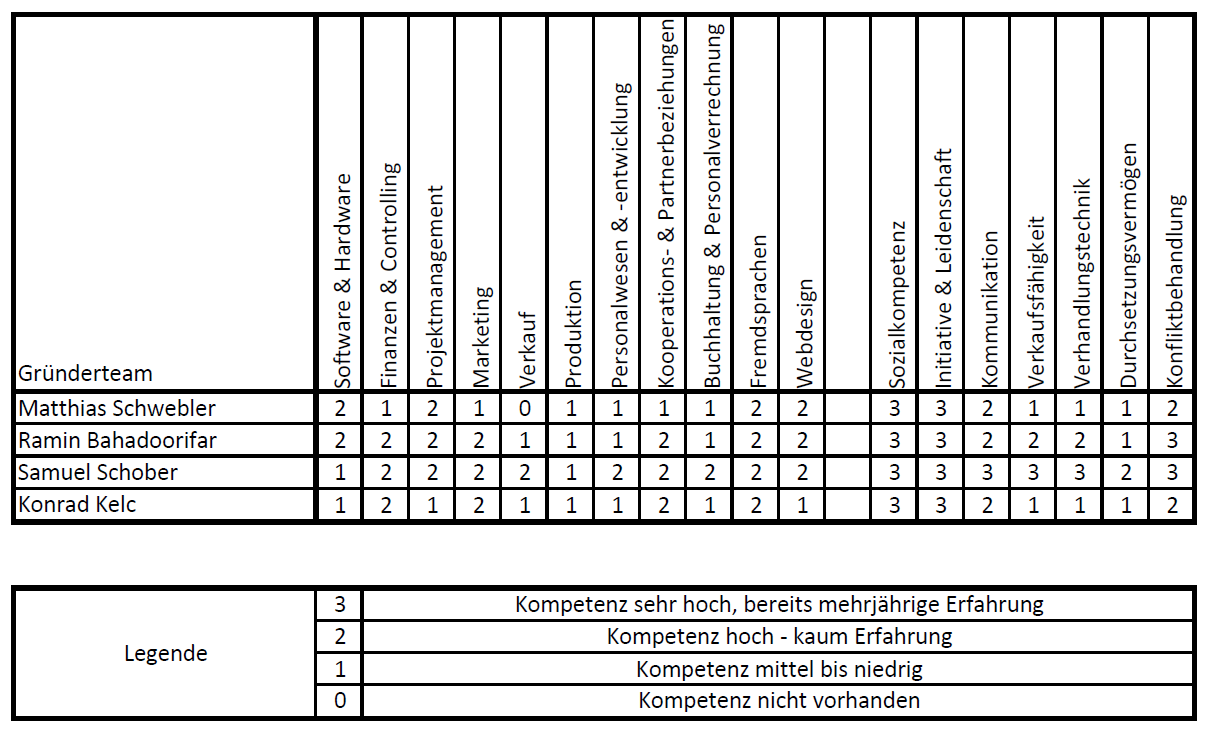
\includegraphics[width=12cm]{faehigkeiten}
\end{center}
\section{Marketing}
\subsection{Gesamtmarkt}

Der Gesamtmarkt f\"ur die Nutzung eines Aquaponic-Systems umfasst Hobbyg\"artner und Personen, die nachhaltig und mit m\"oglichst wenig Aufwand ihre eigenen Kr\"auter und ihr eigenes Gem\"use in der Wohnung anpflanzen wollen. Diese werden in weiterer Folge f\"ur den Hauptmarkt \"Osterreich mit ber\"ucksichtigt.

\subsubsection{\"Osterreich}

Da in \"Osterreich eine magere Marktsituation vorherrscht, und der globale Trend immer mehr in Richtung umweltfreundlicher \"Okosysteme neigt, bietet dieses Projekt eine ideale Vermarktungschance in \"Osterreich.

\subsection{Branchenstruktur und Wettbewerber}

Das Unternehmen Urban Green ist im Bereich umweltfreundliche \"Okosysteme und nachhaltige Nahrungserzeugung t\"atig. Dadurch können wir evtl. Förderungen vom Staat Österreich beantragen, welche für die Entwicklung unseres Produktes viel beisteuern würden.

\subsection{Zielmarkt}

Aufgrund der Natur des Gesch\"aftsmodells ergeben sich zwei Typen von Kunden, denen wir unterschiedliche M\"oglichkeiten bieten k\"onnen:

\clearpage

\subsubsection{Kunden als Besitzer}

Folgende Tabelle zeigt die prim\"ar angesprochenen Kundengruppen in diesem Segment, wobei auch Personen mit wenig bis garkeine Erfahrung in Pflanzenzucht bei einer entsprechenden Bekanntheit von Urban Green als Kunde infrage kommen k\"onnten.

\begin{center}
\begin{tabulary}{\columnwidth}{| p{3cm} | p{4cm} | p{4.3cm} |}
\hline
\textbf{Kundengruppe} & \textbf{Beispiele} & \textbf{Nutzen}\\
\hline
\textbf{Hobbyg\"artner} & Jede Person, die gerne hobbym\"aßig Pflanzen z\"uchtet & OHNE Aufwand Einsicht auf Sensordaten inkl. aufgezeigter M\"oglichkeiten der Verbesserung; Spaß und Motivation durch Erfolgserlebnisse bei der Pflanzenzucht.\\
\hline
\textbf{Vereine Verb\"ande Gruppen} & Aquaponic-Vereine
Kleing\"artnereien
Bio/Vegetarische Ern\"ahrungstreffen & Erfahrungen und Tipps können ausgetauscht werden, usw.\\
\hline
\end{tabulary}
\end{center}

\subsubsection{Kunden als Marketingpartner}


\begin{tabulary}{\columnwidth}{| J | J | J |}
\hline
\textbf{Kundengruppe} & \textbf{Beispiele} & \textbf{Nutzen}\\
\hline
\textbf{Firmen} & Gem\"use und Fischzucht Betriebe, usw. & Firmen- und Kundenevents; Imagebildung durch Werbung \\
\hline
\textbf{Werber im Bereich Bio-Nahrung und nachhaltige Nahrungserzeugung } & Alle Firmen m\"oglich & Ansprechen der Zielgruppen z.B. Hobbyg\"artner, usw; Imagebildung\\
\hline
\end{tabulary}

\subsubsection{Finanziell bedeutendste Kundengruppen}

Die finanziell bedeutendste Kundengruppe sind Hobbyg\"artner und Fischfreunde, welche nicht
die M\"oglichkeiten haben diese Leidenschaften voll auszuleben. Hier soll
das Produkt aushelfen, indem der Kunde sich das Aquaponic System
in der Wohnung installiert und so beide Bed\"urfnisse erf\"ullen kann.

Die zweite sehr bedeutende Kundengruppe sind die Firmenkunden, da diese erstens als Sponsoren dienen sollen. Zweitens erwarten wir uns Einnahmen aus Onlinewerbung , welche von Firmenkunden erbracht werden.

\subsection{Marketingstrategie}

\begin{tabulary}{\columnwidth}{| J | J | J |}
\hline
\textbf{Produkt / Dienstleistung} & \textbf{Produkt / Dienstleistung} & \textbf{Ziel der Produktstrategie}\\
\hline
\textbf{Wartung \& Support} & 48h Wartung & Reibungslose Funktionalit\"at des Produkts \\
\hline
\textbf{Mobiltelefone} & Web-App
mit Grundfunktionalit\"at & Innovationen generieren, kontinuierliche Entwicklungsarbeit \\
\hline
\end{tabulary}

\section{Realisierungsfahrplan}
In diesem Kapitel wird der aktuelle Status der technischen Entwicklung f\"ur die kommenden Monate erl\"autert.

\subsection{Status der technischen Entwicklung}

Das Projekt befindet sich in der Entwicklungsphase. Die verwendete Hard- und Software
wird vom Partner "Ponix Systems" zur Verf\"ugung gestellt.

\subsubsection{Web-App}

Die Grundfunktionalit\"at der Web-App wurde bereits erfolgreich entwickelt. Bis zur Fertigstellung des Projektes erfolgen noch die grafische Aufbereitung der Inhalte sowie umfangreiche Tests, um Fehler erkennen und in weiterer Folge beheben zu k\"onnen.

\subsubsection{Datenbank}

Das verwendete Datenbankmanagementsystem wurde bereits evaluiert und dess Schnittstelle zum Erfassen und Speichern der Daten z.B Sensordaten usw. implementiert.

\subsubsection{Sensoren}

Folgende Sensoren werden im System verwendet:

\begin{itemize}
	\item Temperatursensor
	\item PH-Sensor
	\item EC-Sensor
\end{itemize}

Die Sensoren k\"onnen bereits erfolgreich angesprochen und die Daten abgelesen werden.

\section{Risiken}

Die folgende Abbildung zeigt die Risiken, mit denen Urban Green umzugehen hat und beinhaltet die zentralen Pr\"aventionsma{\ss}nahmen. Damit k\"onnen die Risiken entweder vermindert oder sogar vermieden werden. Das grö{\ss}te Risiko am Scheitern des Urban Green Business Case sind fehlende bzw. unzureichende Finanzierungsquellen, um die technische und kaufm\"annische Entwicklung weiterzuf\"uhren.\\

\begin{center}
	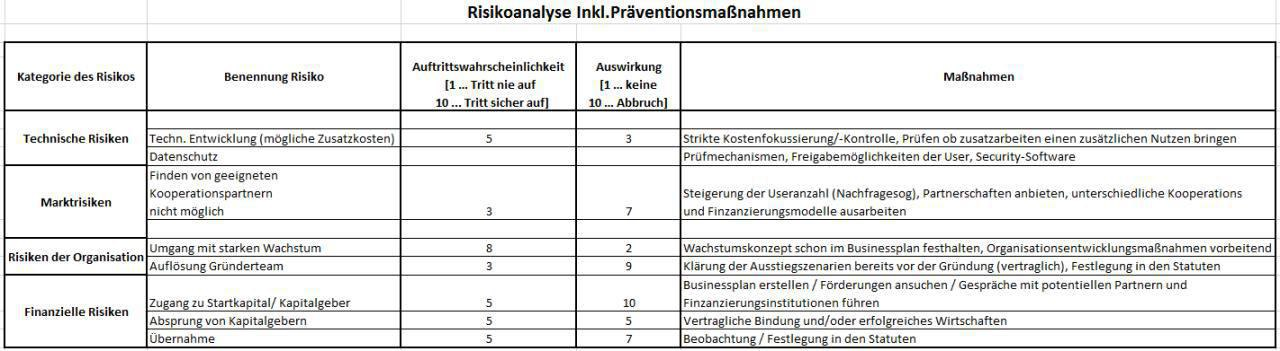
\includegraphics[angle=90,width=5.3cm]{risiken}
\end{center}

\section{Finanzierung}

Da die Finanzierung durch die Investition von unserem Kooperationspartner abhängig ist und uns die Kosten, der zu Verfügung gestellten Materialien und Geräte, noch nicht mitgeteilt wurden, befindet sich dieser Punkt noch in der Evaluierung.

\newpage
\section{Aufteilung}
\begin{table}[ht]
	\centering
	\begin{tabular}{|l|l|lll}
		\cline{1-2}
		\multicolumn{1}{|c|}{\textbf{\rule{0pt}{3ex} Thema}} & \multicolumn{1}{c|}{\textbf{Name}} &  &  &  \\ \cline{1-2}

		\rule{0pt}{3ex} Executive Summary                    & Samuel Schober                     &  &  &  \\ \cline{1-2}
		\rule{0pt}{3ex} Produktidee                          & Matthias Schwebler                 &  &  &  \\ \cline{1-2}
		\rule{0pt}{3ex} Unternehmerteam                      & Matthias Schwebler                 &  &  &  \\ \cline{1-2}
		\rule{0pt}{3ex} Marketing                            & Konrad Kelc                        &  &  &  \\ \cline{1-2}
		\rule{0pt}{3ex} Gesch\"aftssystem und Org.           & Samuel Schober                     &  &  &  \\ \cline{1-2}
		\rule{0pt}{3ex} Realisierungsfahrplan                & Konrad Kelc                        &  &  &  \\ \cline{1-2}
		\rule{0pt}{3ex} Risiken                              & Ramin Bahadoorifar                 &  &  &  \\ \cline{1-2}
		\rule{0pt}{3ex} Finanzierung                         & Ramin Bahadoorifar                 &  &  &  \\ \cline{1-2}
	\end{tabular}
	\caption{Aufteilung}
\end{table}


\end{document}
